    \documentclass[conference]{IEEEtran}
    \IEEEoverridecommandlockouts
    % The preceding line is only needed to identify funding in the first footnote. If that is unneeded, please comment it out.
    \usepackage{cite}
    \usepackage{amsmath,amssymb,amsfonts}
    \usepackage{algorithmic}
    \usepackage{graphicx}
    \usepackage{textcomp}
    \usepackage{xcolor}
    \usepackage{placeins}
    \renewcommand{\abstractname}{Resumen}
    \renewcommand{\refname}{Referencias}
    \renewcommand{\IEEEkeywordsname}{Palabras claves}
    \def\BibTeX{{\rm B\kern-.05em{\sc i\kern-.025em b}\kern-.08em
        T\kern-.1667em\lower.7ex\hbox{E}\kern-.125emX}}
    \begin{document}

    \title{Conference Paper Title}

    \author{\IEEEauthorblockN{1\textsuperscript{st} Fabricio Alonso Lanche Pacsi}
    \IEEEauthorblockA{\textit{dept. Computación} \\
    \textit{Ciencias de la Computación}\\
    Lima, Perú \\
    fabricio.lanche@utec.edu.pe}
    \and
    \IEEEauthorblockN{2\textsuperscript{nd} Jhogan Haldo Pachacutec Aguilar}
    \IEEEauthorblockA{\textit{dept. Computación} \\
    \textit{Ciencias de la Computación}\\
    Lima, Perú\\
    jhogan.pachacutec@utec.edu.pe}
    \and
    \IEEEauthorblockN{3\textsuperscript{rd} Anyeli Azumi Tamara Ureta}
    \IEEEauthorblockA{\textit{dept. Computación} \\
    \textit{Ciencias de la Computación}\\
    Lima, Perú \\
    anyeli.tamara@utec.edu.pe}
    \and
    \IEEEauthorblockN{4\textsuperscript{th} Paulo Ismael Miranda Barrientos}
    \IEEEauthorblockA{\textit{dept. Computación} \\
    \textit{Ciencias de la Computación}\\
    Lima, Perú \\
    paulo.miranda@utec.edu.pe}
    \and
    \IEEEauthorblockN{5\textsuperscript{th} Christofer Renato Perez Torres}
    \IEEEauthorblockA{\textit{dept. Computación} \\
    \textit{Ciencias de Datos}\\
    Lima, Perú \\
    christopher.perez@utec.edu.pe}
    }

    \maketitle

    \begin{abstract}
    This document is a model and instructions for \LaTeX.
    This and the IEEEtran.cls file define the components of your paper [title, text, heads, etc.]. *CRITICAL: Do Not Use Symbols, Special Characters, Footnotes, 
    or Math in Paper Title or Abstract.
    \end{abstract}

    \begin{IEEEkeywords}
    component, formatting, style, styling, insert
    \end{IEEEkeywords}

    \section{Introducción y formulación del problema}

    \subsection{Motivación y relevancia del problema}

    \subsection{Objetivo y tarea de Machine Learning}

    \subsection{Preguntas de investigación e hipótesis}

    \section{Datos y Análisis Exploratorio de Datos (EDA)}

    \subsection{Descripción del dataset}

    \subsection{Variables y variable objetivo}
 
    \subsection{Valores faltantes}

    \FloatBarrier

    El conjunto de datos presenta datos faltantes en 6 de sus 49 variables, lo que afecta al 57.20\% de las observaciones (1,452,912 de 2,540,047). La Tabla~\ref{tab:faltantes} desglosa la cantidad y el origen de los faltantes por variable.

    \begin{table}[h!]
    \centering
    \caption{Valores faltantes por columna.}
    \label{tab:faltantes}
    \begin{tabular}{lrrl}
    \hline
    \textbf{Columna} & \textbf{Faltantes} & \textbf{\%} & \textbf{Origen} \\
    \hline
    \texttt{is\_ftp\_login} & 1,430,065 & 56.30 & Estructural (FTP) \\
    \texttt{ct\_ftp\_cmd}    & 1,429,879 & 56.29 & Estructural (FTP) \\
    \texttt{ct\_flw\_http\_mthd} & 1,348,145 & 53.08 & Estructural (HTTP) \\
    \texttt{dsport}          & 304       & 0.01  & Token corrupto \\
    \texttt{sport}           & 8         & 0.00  & Token corrupto \\
    \texttt{state}           & 8         & 0.00  & Token corrupto \\
    \hline
    \end{tabular}
    \end{table}

    Las tres variables con la mayor proporción de datos faltantes están asociadas al servicio de la conexión. Cada flujo del dataset está etiquetado con su protocolo de aplicación en la variable \texttt{service} (por ejemplo, \texttt{http}, \texttt{ftp} o \texttt{dns}), y \texttt{is\_ftp\_login} y \texttt{ct\_ftp\_cmd} solo tienen sentido en sesiones FTP, mientras que \texttt{ct\_flw\_http\_mthd} solo lo tiene en sesiones HTTP. 

    Los faltantes restantes se concentran en \texttt{sport} (8), \texttt{dsport} (304) y \texttt{state} (8) y representan menos del 0.02\% de las filas. Se originan en tokens corruptos de la fuente original, como literales hexadecimales ilegibles en los puertos y la cadena \texttt{"no"} en \texttt{state}, que fueron interpretados intencionalmente como \texttt{NaN} durante la carga. 

    \subsection{Distribución de clases}

    \FloatBarrier

    La variable objetivo \texttt{attack\_cat} define una tarea multiclase de
    11 clases, las 10 familias de ataque de UNSW-NB15 más la clase
    \texttt{Benign}. Esta última es una clase artificial, no forma parte de
    la taxonomía original del dataset, se construyó agrupando los registros de
    tráfico normal que en la fuente no presentan una categoría de ataque
    definida y que el indicador binario \texttt{Label} marca como no ataque
    (0). La verificación sobre los datos confirma que ambas definiciones
    coinciden al 100\%.

    La Tabla~\ref{tab:descriptivos} resume los estadísticos de las variables
    numéricas y permite una lectura global de las características. Muchas
    presentan distribuciones extremas, con medias muy superiores a sus
    medianas, como \texttt{Sload} (36.96M frente a 589,304), \texttt{Sjit}
    (1,589 frente a 19.12) o \texttt{Sintpkt} (193 frente a 0.47), y otras
    están fuertemente infladas en cero, como \texttt{trans\_depth} (91.9\%),
    \texttt{res\_bdy\_len} (92.7\%) y \texttt{ct\_state\_ttl} (85.8\%). Estas
    características se relacionan directamente con los conteos de outliers
    descritos más adelante.

    \begin{table}[h!]
    \centering
    \caption{Estadísticos descriptivos de las variables numéricas.}
\label{tab:descriptivos}
\resizebox{\columnwidth}{!}{%
\begin{tabular}{lrrrrrr}
\hline
\textbf{Variable} & \textbf{Media} & \textbf{Mediana} & \textbf{Q1} & \textbf{Q3} & \textbf{Mín} & \textbf{Máx} \\
\hline
\texttt{sport} & 30,535 & 31,687 & 11,226 & 47,439 & 0.00 & 65,535 \\
\texttt{dsport} & 11,235 & 80.00 & 53.00 & 14,970 & 0.00 & 65,535 \\
\texttt{dur} & 0.66 & 0.02 & 0.0010 & 0.21 & 0.00 & 8,787 \\
\texttt{sbytes} & 4,340 & 1,470 & 200.00 & 3,182 & 0.00 & 1.436e+07 \\
\texttt{dbytes} & 36,428 & 1,820 & 178.00 & 14,894 & 0.00 & 1.466e+07 \\
\texttt{sttl} & 62.78 & 31.00 & 31.00 & 31.00 & 0.00 & 255.00 \\
\texttt{dttl} & 30.77 & 29.00 & 29.00 & 29.00 & 0.00 & 254.00 \\
\texttt{sloss} & 5.16 & 3.00 & 0.00 & 7.00 & 0.00 & 5,319 \\
\texttt{dloss} & 16.33 & 4.00 & 0.00 & 14.00 & 0.00 & 5,507 \\
\texttt{Sload} & 3.696e+07 & 589,304 & 135,396 & 2,039,923 & 0.00 & 5.988e+09 \\
\texttt{Dload} & 2,450,861 & 589,318 & 11,916 & 2,925,974 & 0.00 & 1.288e+08 \\
\texttt{Spkts} & 33.29 & 12.00 & 2.00 & 44.00 & 0.00 & 10,646 \\
\texttt{Dpkts} & 42.73 & 12.00 & 2.00 & 42.00 & 0.00 & 11,018 \\
\texttt{swin} & 150.09 & 255.00 & 0.00 & 255.00 & 0.00 & 255.00 \\
\texttt{dwin} & 149.75 & 255.00 & 0.00 & 255.00 & 0.00 & 255.00 \\
\texttt{stcpb} & 1.262e+09 & 6.397e+08 & 0.00 & 2.467e+09 & 0.00 & 4.295e+09 \\
\texttt{dtcpb} & 1.262e+09 & 6.384e+08 & 0.00 & 2.469e+09 & 0.00 & 4.295e+09 \\
\texttt{smeansz} & 124.25 & 73.00 & 60.00 & 132.00 & 0.00 & 1,504 \\
\texttt{dmeansz} & 276.67 & 89.00 & 69.00 & 565.00 & 0.00 & 1,500 \\
\texttt{trans\_depth} & 0.08 & 0.00 & 0.00 & 0.00 & 0.00 & 172.00 \\
\texttt{res\_bdy\_len} & 4,242 & 0.00 & 0.00 & 0.00 & 0.00 & 6,558,056 \\
\texttt{Sjit} & 1,589 & 19.12 & 0.00 & 413.79 & 0.00 & 1,483,831 \\
\texttt{Djit} & 730.08 & 2.65 & 0.00 & 63.51 & 0.00 & 781,221 \\
\texttt{Stime} & 1.423e+09 & 1.424e+09 & 1.422e+09 & 1.424e+09 & 1.422e+09 & 1.424e+09 \\
\texttt{Ltime} & 1.423e+09 & 1.424e+09 & 1.422e+09 & 1.424e+09 & 1.422e+09 & 1.424e+09 \\
\texttt{Sintpkt} & 193.32 & 0.47 & 0.0090 & 7.35 & 0.00 & 84,371 \\
\texttt{Dintpkt} & 78.82 & 0.41 & 0.0060 & 6.20 & 0.00 & 59,485 \\
\texttt{tcprtt} & 0.0062 & 0.0006 & 0.00 & 0.0007 & 0.00 & 10.04 \\
\texttt{synack} & 0.0033 & 0.0005 & 0.00 & 0.0006 & 0.00 & 4.53 \\
\texttt{ackdat} & 0.0029 & 0.0001 & 0.00 & 0.0001 & 0.00 & 5.51 \\
\texttt{ct\_state\_ttl} & 0.26 & 0.00 & 0.00 & 0.00 & 0.00 & 6.00 \\
\texttt{ct\_flw\_http\_mthd} & 0.23 & 0.00 & 0.00 & 0.00 & 0.00 & 36.00 \\
\texttt{ct\_ftp\_cmd} & 0.05 & 0.00 & 0.00 & 0.00 & 0.00 & 8.00 \\
\texttt{ct\_srv\_src} & 9.21 & 5.00 & 2.00 & 10.00 & 1.00 & 67.00 \\
\texttt{ct\_srv\_dst} & 8.99 & 5.00 & 2.00 & 10.00 & 1.00 & 67.00 \\
\texttt{ct\_dst\_ltm} & 6.44 & 3.00 & 2.00 & 6.00 & 1.00 & 67.00 \\
\texttt{ct\_src\_ltm} & 6.90 & 4.00 & 2.00 & 7.00 & 1.00 & 67.00 \\
\texttt{ct\_src\_dport\_ltm} & 4.64 & 1.00 & 1.00 & 2.00 & 1.00 & 67.00 \\
\texttt{ct\_dst\_sport\_ltm} & 3.59 & 1.00 & 1.00 & 1.00 & 1.00 & 60.00 \\
\texttt{ct\_dst\_src\_ltm} & 6.85 & 2.00 & 1.00 & 5.00 & 1.00 & 67.00 \\
\hline
\end{tabular}}
\end{table}

    \begin{figure}[h!]
    \centering
    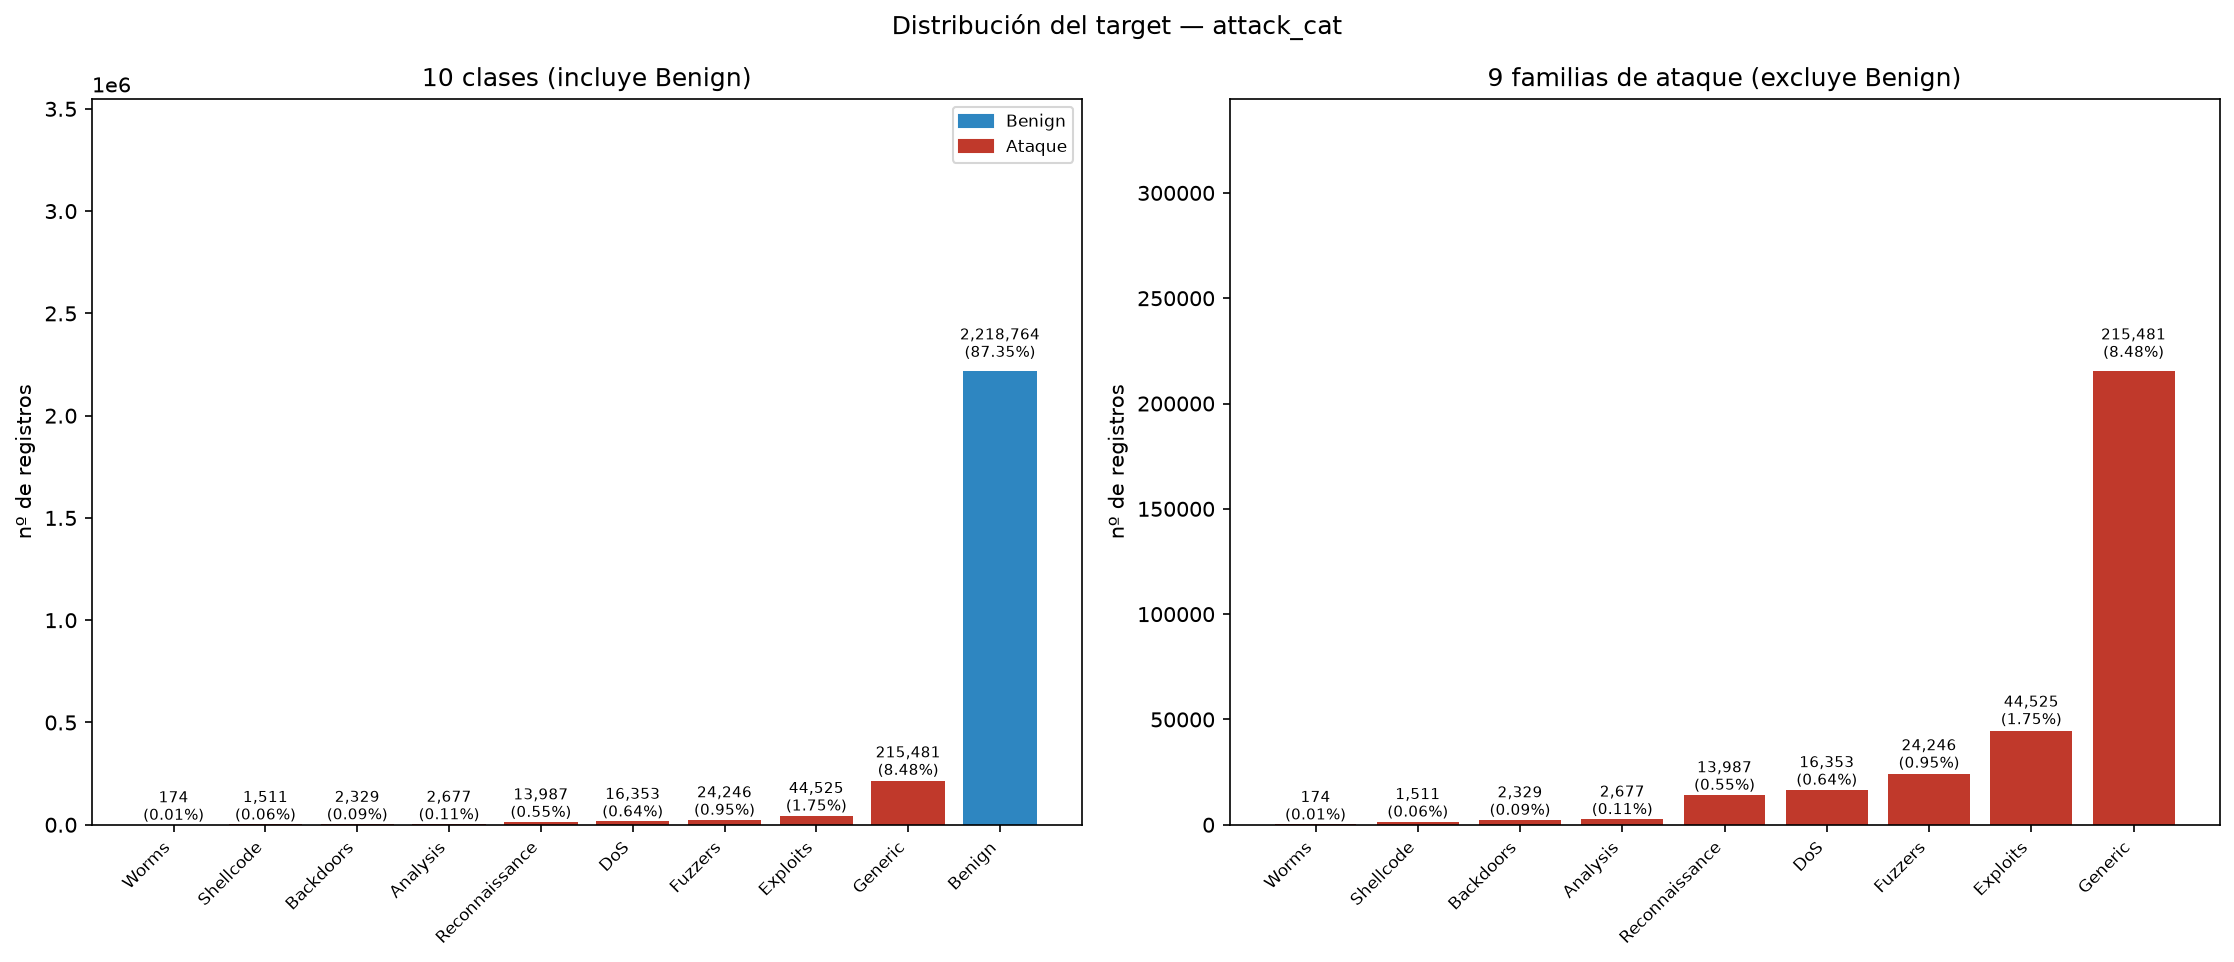
\includegraphics[width=\columnwidth]{output/fig01_distribucion_clases.png}
    \caption{Distribución del target por clase (escala logarítmica).}
    \label{fig:clases}
    \end{figure}

    La Fig.~\ref{fig:clases} presenta la distribución del target en las 11
    clases, en escala logarítmica. El target presenta un fuerte desbalance. La clase \texttt{Benign}
    concentra el 87.35\% de los registros y las clases de ataque apenas el
    12.65\%, repartidas de forma muy desigual. \texttt{Generic} reúne la
    mayor parte de los ataques, 215,481 registros (8.48\% del total, dos
    tercios de los ataques), mientras que \texttt{Worms} cuenta con solo 174
    registros (0.007\%). En el plano binario, la proporción Benign frente a
    ataque es de aproximadamente 7:1. Este desbalance condicionará la
    elección de métricas de evaluación y el tratamiento de las clases
    minoritarias en la fase de modelado.

    \subsection{Problemas de calidad y outliers}

    \FloatBarrier

    El dataset presenta 480,633 filas duplicadas, un 18.92\% del total. Se trata de duplicados exactos, mismos valores de características y mismo target, que no aportan información adicional y resultan candidatos a eliminación durante el preprocesamiento. No se identificaron columnas constantes.

    La cardinalidad de las variables nominales es heterogénea, como se resume en la Tabla~\ref{tab:cardinalidad}. Las direcciones IP \texttt{srcip} y \texttt{dstip} registran 43 y 47 valores únicos respectivamente, una diversidad inusualmente baja para campos de este tipo que sugiere pocos hosts en el escenario de captura. Los puertos \texttt{sport} y \texttt{dsport} presentan cardinalidad alta, con cerca de 65 mil valores únicos (2.5\% del total). El resto de las nominales se limita a pocas categorías.

    \begin{table}[h!]
    \centering
    \caption{Cardinalidad de las variables nominales.}
    \label{tab:cardinalidad}
    \begin{tabular}{lrr}
    \hline
    \textbf{Variable} & \textbf{Valores únicos} & \textbf{\%} \\
    \hline
    \texttt{srcip}   & 43      & 0.002 \\
    \texttt{dstip}   & 47      & 0.002 \\
    \texttt{sport}   & 64,598  & 2.543 \\
    \texttt{dsport}  & 64,627  & 2.544 \\
    \texttt{proto}   & 135     & 0.005 \\
    \texttt{state}   & 16      & 0.001 \\
    \texttt{service} & 13      & 0.001 \\
    \hline
    \end{tabular}
    \end{table}

    Para cuantificar los valores atípicos se aplicó el criterio del rango
    intercuartílico, que considera atípico todo valor fuera del intervalo
    $[Q_1-1.5\,\mathrm{IQR},\ Q_3+1.5\,\mathrm{IQR}]$. Bajo este criterio, una
    fracción elevada de las variables numéricas presenta valores atípicos
    (Tabla~\ref{tab:outliers}), pero estos conteos reflejan la forma de las
    distribuciones más que datos corruptos, se concentran en variables de cola
    larga y fuertemente infladas en cero, como \texttt{Sload} (22.17\%),
    \texttt{Sjit} (18.63\%, con 37.93\% de ceros), \texttt{dur} (17.77\%) o
    \texttt{Dintpkt} (17.86\%, con 19.71\% de ceros). Las variables acotadas,
    como los campos TTL, y la mayoría de los contadores \texttt{ct\_*}, no
    presentan outliers.

    \begin{table}[h!]
    \centering
    \caption{Outliers por IQR y proporción de ceros en variables numéricas seleccionadas.}
    \label{tab:outliers}
    \begin{tabular}{lrr}
    \hline
    \textbf{Variable} & \textbf{\% outliers} & \textbf{\% ceros} \\
    \hline
    \texttt{Sload}          & 22.17 & 0.20  \\
    \texttt{ct\_src\_dport\_ltm} & 21.01 & 0.00  \\
    \texttt{Sjit}           & 18.63 & 37.93 \\
    \texttt{Dintpkt}        & 17.86 & 19.71 \\
    \texttt{dur}            & 17.77 & 0.33  \\
    \texttt{Sintpkt}        & 17.56 & 0.06  \\
    \hline
    \end{tabular}
    \end{table}

    La Fig.~\ref{fig:boxplot} complementa esta lectura mediante boxplots en
    escala logarítmica, que despliegan la dispersión de las variables
    numéricas clave y marcan explícitamente los outliers (fliers) que los
    conteos por IQR cuantifican.

    \begin{figure}[h!]
    \centering
    
\includegraphics[width=\columnwidth]{output/fig06b_boxplot.png}
    \caption{Boxplot en escala logarítmica de las variables numéricas clave con outliers destacados.}
    \label{fig:boxplot}
    \end{figure}

    \FloatBarrier

    \subsection{Relaciones entre variables (correlaciones)}

    La Fig.~\ref{fig:correlacion} presenta la matriz de correlación de
    Pearson entre las variables numéricas y el target binario (tráfico
    normal frente a ataque). La mayoría de las variables guarda con el target
    una correlación débil o moderada, con excepción de \texttt{sttl} (0.90) y
    \texttt{ct\_state\_ttl} (0.87), cuya interpretación se analiza en la
    siguiente subsección. Entre las variables con mayor correlación positiva
    moderada figuran \texttt{Sload} (0.19), \texttt{ackdat} y \texttt{tcprtt}
    (0.14), mientras que \texttt{Dload} ($-0.22$) presenta la mayor
    correlación negativa.

    \begin{figure}[h!]
    \centering
    
\includegraphics[width=\columnwidth]{output/fig04_correlacion_features.png}
    \caption{Correlación de Pearson entre las variables numéricas y el target binario.}
    \label{fig:correlacion}
    \end{figure}

    La Fig.~\ref{fig:hist} complementa el análisis de correlaciones al
    comparar, clase por clase, la distribución de las variables numéricas
    clave, las diferencias entre el tráfico benigno y las conexiones de
    ataque permiten identificar qué variables separan mejor ambas
    poblaciones y cuáles presentan distribuciones prácticamente idénticas.

    \begin{figure}[h!]
    \centering
    
\includegraphics[width=\columnwidth]{output/fig06_histogramas_num.png}
    \caption{Distribución de variables numéricas clave según la clase (muestra de 200 mil registros).}
    \label{fig:hist}
    \end{figure}

    Por el lado de la redundancia, numerosos pares de variables están
    altamente correlacionados entre sí y transmiten información duplicada,
    como \texttt{Stime} y \texttt{Ltime} (1.00), \texttt{swin} y \texttt{dwin}
    (0.997), \texttt{dbytes} con \texttt{dloss} (0.99) y \texttt{Dpkts} (0.97),
    y \texttt{sbytes} con \texttt{sloss} (0.96). Entre los contadores de
    ventana \texttt{ct\_*} las correlaciones también son altas, con valores
    superiores a 0.9 en varios pares. Este patrón indica redundancia en el
    espacio de características, que deberá tenerse en cuenta al definir la
    lista de predictores. En particular, los contadores de ventana
    \texttt{ct\_*} presentan las correlaciones más altas con el target en
    todo el conjunto, con \texttt{ct\_state\_ttl} (0.874) y
    \texttt{ct\_dst\_src\_ltm} (0.440) a la cabeza, como detalla la
    Fig.~\ref{fig:ct_corr}. La interpretación de estos valores y su posible
    implicación como fuga de información se retomará en la sección de sesgo
    y data leakage.

    \begin{figure}[h!]
    \centering
    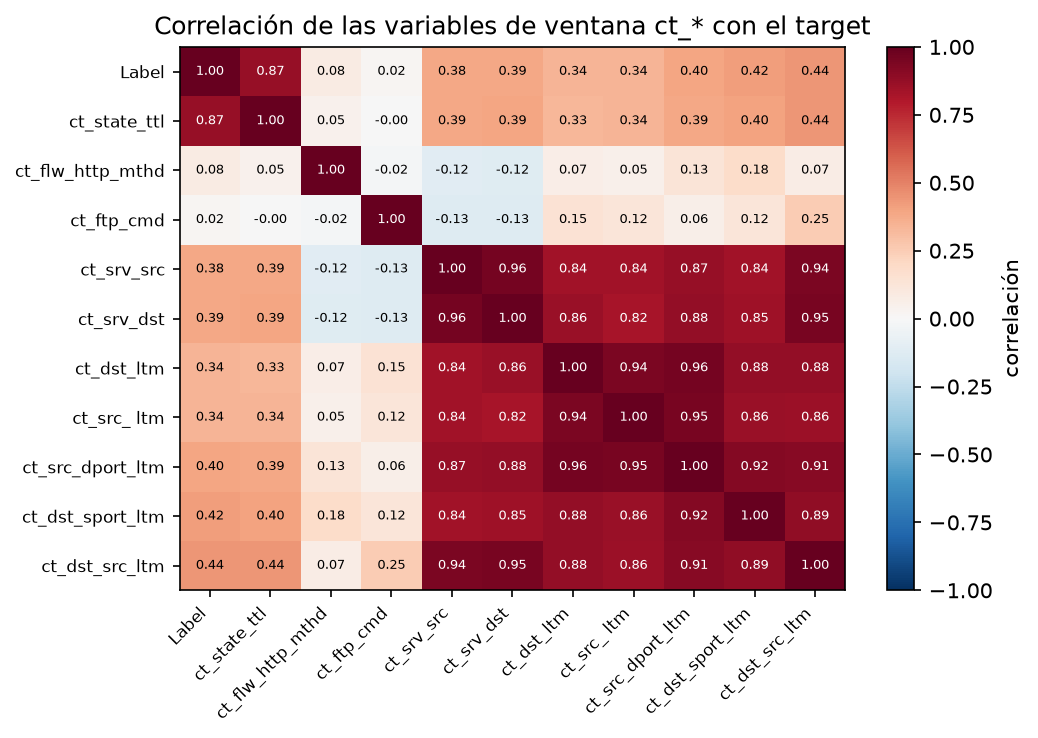
\includegraphics[width=\columnwidth]{output/fig05_ct_vs_target.png}
    \caption{Correlación de las variables de ventana \texttt{ct\_*} con el target.}
    \label{fig:ct_corr}
    \end{figure}

    \subsection{Sesgo y data leakage}

    \begin{thebibliography}{00}
    \bibitem{b1} G. Eason, B. Noble, and I. N. Sneddon, ``On certain integrals of Lipschitz-Hankel type involving products of Bessel functions,'' Phil. Trans. Roy. Soc. London, vol. A247, pp. 529--551, April 1955.
    \bibitem{b2} J. Clerk Maxwell, A Treatise on Electricity and Magnetism, 3rd ed., vol. 2. Oxford: Clarendon, 1892, pp.68--73.
    \bibitem{b3} I. S. Jacobs and C. P. Bean, ``Fine particles, thin films and exchange anisotropy,'' in Magnetism, vol. III, G. T. Rado and H. Suhl, Eds. New York: Academic, 1963, pp. 271--350.
    \bibitem{b4} K. Elissa, ``Title of paper if known,'' unpublished.
    \bibitem{b5} R. Nicole, ``Title of paper with only first word capitalized,'' J. Name Stand. Abbrev., in press.
    \bibitem{b6} Y. Yorozu, M. Hirano, K. Oka, and Y. Tagawa, ``Electron spectroscopy studies on magneto-optical media and plastic substrate interface,'' IEEE Transl. J. Magn. Japan, vol. 2, pp. 740--741, August 1987 [Digests 9th Annual Conf. Magnetics Japan, p. 301, 1982].
    \bibitem{b7} M. Young, The Technical Writer's Handbook. Mill Valley, CA: University Science, 1989.
    \end{thebibliography}

    \end{document}
